% !TeX root = ../report_project_2stage_OTA.tex

\section{Specifications and Architecture}

\subsection{Initial Design Specifications}

The OTA is intended for a low-power PMIC or voltage-reference application.
The design therefore prioritizes DC gain, low current consumption, stability
and supply rejection over maximum speed.

The initial design targets are summarized in
Table~\ref{tab:initial_specs}.

\begin{table}[ht]
    \centering
    \caption{Initial OTA design specifications.}
    \label{tab:initial_specs}
    \begin{tabular}{ll}
        \hline
        Parameter & Initial target \\
        \hline
        Supply voltage & 1.8 V \\
        DC gain & $\geq 80$ dB \\
        GBW & $\geq 1$ MHz \\
        Phase margin & $\geq 60^\circ$ \\
        Load capacitance & 2 pF nominal, 4 pF maximum \\
        Quiescent current & Minimize within the other constraints \\
        PSRR & High priority, characterized versus frequency \\
        Slew rate & Secondary design objective \\
        \hline
    \end{tabular}
\end{table}


\subsection{Selected Topology}

A classical two-stage Miller-compensated CMOS OTA is selected.

The first stage uses a PMOS differential pair with an NMOS
current-mirror active load. Its single-ended output node,
\texttt{out\_s1}, drives the second stage.

The second stage consists of the NMOS common-source transistor
\texttt{NLOAD\_2}, biased by the PMOS current source
\texttt{PTAIL\_2}. The OTA output is denoted \texttt{Vout}.

The compensation network is connected between \texttt{out\_s1}
and \texttt{Vout}. It contains the Miller capacitor
\texttt{CMILLER} and, when required, the series resistor
\texttt{RMILLER}.


\begin{figure}[ht]
    \centering
    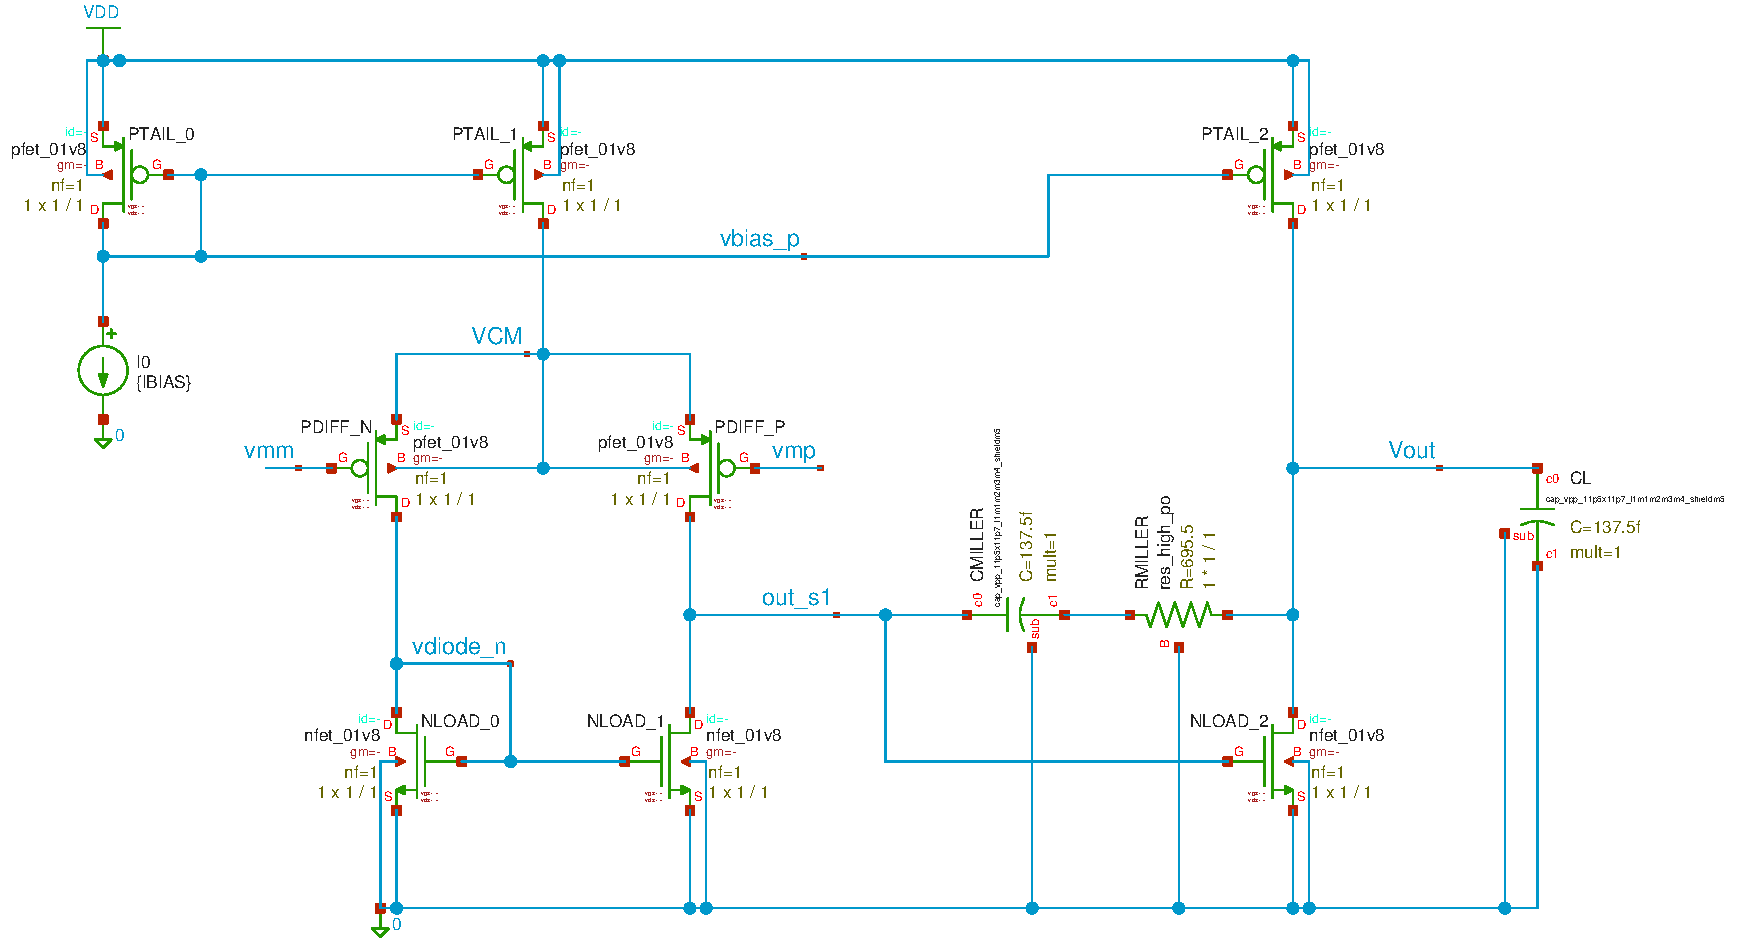
\includegraphics[width=\textwidth]
    {figures/transistor/schematics/ota_2stage_topology.pdf}
    \caption{Selected two-stage OTA topology and device naming convention.}
    \label{fig:ota_topology}
\end{figure}


\subsection{Device Naming}

The naming convention shown in Figure~\ref{fig:ota_topology} is used
throughout the analytical design and simulation results.

\begin{itemize}
    \item \texttt{PTAIL\_0}: diode-connected PMOS receiving the reference
    bias current and generating the PMOS mirror bias voltage,

    \item \texttt{PTAIL\_1}: PMOS current source biasing the first stage,

    \item \texttt{PDIFF\_P}, \texttt{PDIFF\_N}: PMOS input differential pair,

    \item \texttt{NLOAD\_0}, \texttt{NLOAD\_1}: NMOS current-mirror
    active load,

    \item \texttt{out\_s1}: first-stage output and second-stage input,

    \item \texttt{PTAIL\_2}: PMOS current source biasing the second stage,

    \item \texttt{NLOAD\_2}: NMOS common-source transistor of the
    second gain stage,

    \item \texttt{Vout}: OTA output,

    \item \texttt{CMILLER}: Miller compensation capacitor,

    \item \texttt{RMILLER}: optional series compensation resistor.
\end{itemize}


\subsection{Bias-Current Architecture}

The diode-connected device \texttt{PTAIL\_0} defines the reference
current unit $I$.

The first-stage current is initially defined as

\[
I_{\mathrm{PTAIL\_1}} = I,
\]

which gives, at zero differential input,

\[
I_{\mathrm{PDIFF\_P}}
=
I_{\mathrm{PDIFF\_N}}
=
\frac{I}{2}.
\]

The second-stage current is expressed as

\[
I_{\mathrm{PTAIL\_2}} = N I,
\]

where the mirror ratio $N$ is derived from the required second-stage
transconductance and stability constraints in the first-order design.
